\section{Theory}

\subsection{Direct and Indirect Band Gap Semiconductors}

The band gap of a material is the minimum difference in energy between the highest energy state of the valence band and the lowest energy state of the conduction band. However, these values may not occur at the same value of electron momentum. When the top of the valence band and the bottom of the conduction band align at the same value of momentum, the material is called a direct band gap material. Otherwise, it is called an indirect band gap material.

In optical devices, the difference between the two are quite significant. A typical photon energy is of the order of $10^{-19}$ J and since $p=E/c$, it equates to very small momentum. 

In semiconductor devices, a photon of energy $E_g$ can produce an electron-hole pair. In direct band gap materials, the process is much easier since the electron does not need to be given much momentum. But in an indirect band gap semiconductor, the electron must also undergo a significant change in its momentum for a photon of energy $E_g$ to produce the same (Fig. \ref{bg}). This means that in addition to interacting with a photon to gain energy, it also needs to interact with a lattice vibration called a phonon to lose/gain momentum.

This indirect process happens at a slower rate as it requires the interaction of an electron, a photon and a phonon. Since the same principle also applies to recombination of electrons and holes, that process is also faster for direct band gap semiconductors. Even though a broad spectrum of phonons are available in a crystal lattice, those phonons which conserve
the momentum participate for indirect transitions.

\begin{figure}
    \centering
    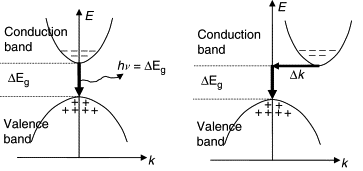
\includegraphics[width=1\columnwidth]{images/bg.png}
    \caption{Illustration of direct bandgap (left) and indirect bandgap (right) of semiconductor materials \cite{HUI20091}.}
    \label{bg}
\end{figure}

\subsection{UV-Vis spectroscopy for optical band gap measurement}
UV-Vis spectroscopy measures light absorption as function of wavelength. It gives information on electronic transitions occurring in semiconductor material and can be used to estimate the optical band gap. 

For a sample of thickness $d$, the absorption coefficient of light $\alpha$ is given by, 

\begin{align} \label{1}
    \alpha \text{ (cm)}^{-1} = \frac{2.303A}{d}
\end{align}

where $A$ is the absorbance of the sample, given by

\begin{align} \label{eq}
    A = \log_{10} \left(\frac{I_0}{I_T}\right)
\end{align}

Here, $I_T$ is the transmitted light and $I_0$ is the incident light, which are related by the Beer-Lambert's law. 
% Specifically, it relates the absorbance ($A$) of a sample to the molar absorptivity coefficient ($\epsilon$), the concentration of the absorbing species ($C$), and the path length of light through the sample ($l$). Absorbance is calculated as the negative logarithm of the ratio of transmitted intensity ($I_T$) to incident intensity ($I_O$). Thus,

\begin{align}
    I_T = I_0 e^{\alpha d}
    % A=\epsilon c l=-\log_{10}\left(\frac{I_T}{I_o}\right)
\end{align}

Energy band gap of a given material can be precisely calculated using \textit{Tauc method} as,

\begin{align}
    \alpha(h\nu) = A(h\nu - E_g)^n
\end{align}

where $n=1/2$ for direct allowed transitions and $n=2$ for indirect allowed transitions \cite{Pankove_1975}. Therefore, for direct band gap materials,

\begin{align} \label{directeq}
    \alpha(h\nu) = A(h\nu - E_g)^{0.5}
\end{align}

Hence they exhibit a sharp rise in absorption above the Eg in the plot of energy of light source of Uv-vis setup versus absorption coefficient $\alpha$. For indirect band gap materials,

\begin{align}
    \alpha(h\nu) = A(h\nu - E_g \pm E_p)^{2}
\end{align}

where $E_p$ refers to the addition energy for the phonon interaction. The sign `+' corresponds to phonon emission, and the sign `-' corresponds to phonon absorption. The band gap is estimated by plotting $\sqrt{\alpha}$ versus energy and finding the intercept of the linear region.

% ======================================================================================
\section{Experimental Setup}

\subsection*{Apparatus}

\begin{enumerate}
    \item A laser lamp
    \item Glass plates
    \item ZnTe, CdS and ZnO coated glass slides
    \item UV-Vis spectroscope and Analysing software
    \item Optical Cables for connection\\
\end{enumerate}

In the experiment, we use a spectrum analyzer software which samples wavelengths from 340 to 1000 nm, which lie in the UV-Vis range. The thin films are held in a sample holder box  through which the light source is passed. To get the corrected spectrum of the sample, we first take a dark measurement with the lights turned off $I_\text{dark}$. Now, we take the spectrum of the empty glass slide as reference ($I_\text{ref}$). Finally, the sample data is taken by placing the sample in front of the light source ($I_\text{sample}$). The final absorbalnce is calculated using Eq. \ref{eq} after subtracting the dark values.

\begin{align}
    A = \log_{10} \left(\frac{I_\text{ref}-I_\text{dark}}{I_\text{sample}-I_\text{dark}}\right)
\end{align}